\subsection{Someone In Charge}

\subsubsection*{Ausgangslage}
Ein System besteht aus mehreren Units of Mitigation (1), kann Redundancy (3) verwenden und verfolgt das Prinzip von Minimize Human Interaction (5).
Dennoch können überall Fehler auftreten, selbst in der Fehlerbehandlung. Tritt dieser Fall ein, kann es sein, dass das System, zusätzlich zum Ausfall der Funktionalität auch noch die Fehlerbehandlung nicht weiterführen kann.

\subsubsection*{Lösungsansatz}

Bei der Fehlertoleranz gibt es zwei Arten der Fehlererkennung:
\begin{enumerate}
	\item Fehler erkennen, der passiert ist (komplexer)
	\item Die Komponente im System finde, welche nicht mehr korrekt funktioniert (einfacher)
\end{enumerate}
Hat ein System eine Komponente, die weiss was bei der Erkennung eines Fehlers gemacht werden muss, führt das zu einem robusteren System. Mindestens sollte diese den Fehler einem Fault Observer (10) oder System Monitor (15) melden können, nebst einer möglichen Fehlerbehandlung. Ein Fault Observer (10) ist zuständig für das Sammeln und Weiterleiten von Informationen von Fehlern, ein System Monitor (15) hingegen erkennt Fehler.
Wichtig ist einfach, dass im Falle eines Fehlers bekannt ist, wer sich darum kümmern muss.
Das Problem dabei ist aber, dass dadurch ein Single Point of Failure entsteht, da diese Komponente auch ausfallen kann. Es ist deshalb nicht definiert, dass es nur eine Komponente geben darf, die reagieren kann. Es ist lediglich definiert, dass zu jedem Zeitpunkt klar sein muss, wer reagieren muss.
Wichtig ist auch zu beachten, dass die verantwortlichen Komponenten sich nicht um zu viel kümmern müssen. Es ist einfacher, wenn sich viele verschieden Komponenten um verschieden Fehlerbehandlungen kümmern, da diese so einfacher wartbar sind und bei einem Ausfall einer Komponenten nicht die gesamte Fehlerbehandlung betroffen ist.

\begin{figure}[H]
	\centering
	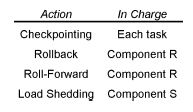
\includegraphics{content/faulttolerance/images/ResponsibilitiesList.JPG}
	\caption{ResponsibilitiesList}
\end{figure}


\subsubsection*{Schlussfolgerung}

Alle Aktivitäten, die fehlertolerant sein müssen, benötigen eine einzige Komponente, die in einem Fehlerfall reagiert.
Es muss auch möglich sein, dass Fehler bei der Fehlerbehandlung erkannt werden können und falls nötig Escalation (9) eingesetzt wird.

\subsubsection*{Verwandte Patterns}

Fehler-„Verwaltung“:
\begin{itemize}
	\item Fault Observer (10)
	\item System Monitor (15)
\end{itemize}

\begin{itemize}
	\item Heartbeats (16)
	\item Acknowledgements (17)
\end{itemize}

\begin{itemize}
	\item Escalation (9)
\end{itemize}

